\subsection{Debug Window Size}
\label{sec:timewindowPerformance}


\begin{table}[ht]
	\centering
	\begin{tabular}{|c|r|r|r|}
		\hline
		{\bf \begin{tabular}[c]{@{}c@{}}Input \\ Rate\end{tabular}} & \multicolumn{1}{c|}{{\bf \begin{tabular}[c]{@{}c@{}}Debug \\ Window\end{tabular}}} & \multicolumn{1}{c|}{{\bf \begin{tabular}[c]{@{}c@{}}Pipe \\ Size\end{tabular}}} & \multicolumn{1}{c|}{{\bf \begin{tabular}[c]{@{}c@{}}Slow- \\ down\end{tabular}}} \\ \hline
		530 bps, 27 rq/s                                            & $\infinity$                                                                                     & 4096                                                                            & 1.8x                                                                             \\ \hline
		530 bps, 27 rq/s                                            & 8 sec                                                                              & 4096                                                                            & 3x                                                                               \\ \hline
		530 bps, 27 rq/s                                            & 72 sec                                                                             & 16384                                                                           & 3x                                                                               \\ \hline
		Poisson, $\lambda$ = 17 rq/s                                        & 16 sec                                                                             & 4096                                                                            & 8x                                                                               \\ \hline
		Poisson, $\lambda$ = 17 rq/s                                        & 18 sec                                                                             & 4096                                                                            & 5x                                                                               \\ \hline
		Poisson, $\lambda$ = 17 rq/s                                        & $\infinity$                                                                                     & 65536                                                                           & 3.2x                                                                             \\ \hline
		Poisson, $\lambda$ = 17 rq/s                                        & 376 sec                                                                            & 16384                                                                           & 3.2x                                                                             \\ \hline
	\end{tabular}
	%\captionsetup{justification=centering}
	\caption{Approximate debug window sizes for a MySQL request workload}
	\label{table:timewindow}
\end{table}

\noindent
\textbf{Experimental Results:} We call the time taken to reach a buffer overflow the ``debug-window'' for the debug-container.
As explained earlier (see section \ref{sec:timewindowPerformance}), the size of this debug-window, depends both on the overhead of the ``instrumentation'', the incoming workload distribution, and the size of the buffer.
To evaluate the approximate size of the debug-window, we sent requests to a production and debug MySQL container via our network duplicator.
Each workload ran for about 7 minutes (10,000 ``select * from table'' queries), with varying request workloads.
We also profiled the server, and found that is able to process a max of 27 req/s\footnote{Not the same as bandwidth, 27 req/s is the maximum rate of sequential requests MySQL server is able to handle for a user session} in a single user connect session. 
For each of our experiments we vary the buffer sizes to get an idea of debug-window. 
Additionally, we generated a slowdown by first modeling the time taken by MySQL to process requests (27 req/s or 17req/s), and then putting an approximate sleep in the request handler.

Initially, we created a connection, and sent requests at the maximum request rate the server was able to handle (27 req/s).
We found that for overheads up-to 1.8x (approx) we experienced no buffer overflows.
% most function tracing and profiling tools generally have an overhead of 1-1.5x for lower granularity and 2x for higher granularity tracing.
For higher overheads the debug window rapidly decreased, with buffer sizes primarily dependent on buffer-size, request size, and slowdown.

Next, we mimic user behavior, to generate a realistic workload.
We send packets using a poisson process with an average request rate of 17 requests per second to our proxy. 
This varies the inter-request arrival time, and let's the cloned debug-container catch up with the production container during idle time-periods in between request bursts.
We observed, that compared to earlier experiments, there was more slack in the system with slightly lesser amount of requests, this meant that our system was able to tolerate much with the default buffer size (linux default pipe size is 65536), the system was able to tolerate a much higher overhead (3.2x) with no buffer overflows.


\begin{figure}[ht]
	%{0.45\textwidth}
	\centering
	%  \resizebox{\linewidth}{!}{
	\begin{adjustbox}{max size={.45\textwidth}}
		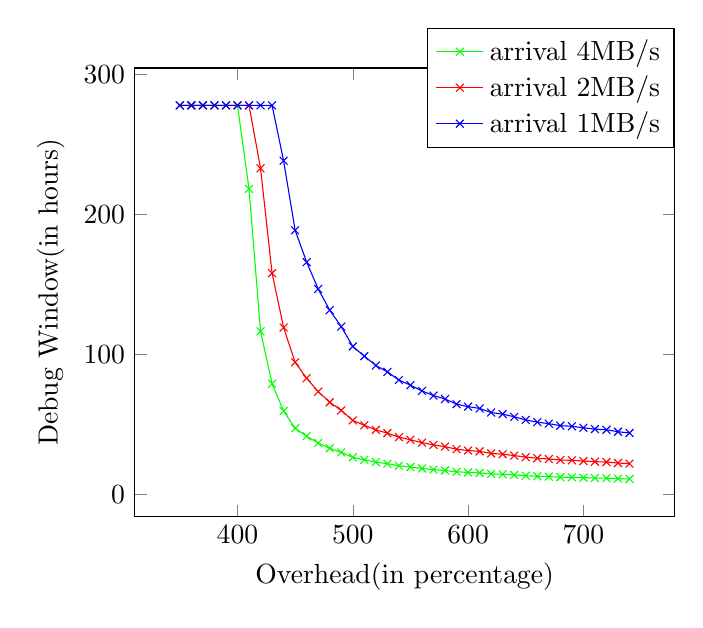
\begin{tikzpicture}
		\begin{axis}[
		%xmode=log,
		legend style={at={(1,1.09)},anchor=north east,legend columns=1},
		xlabel=Overhead(in percentage),
		ylabel=Debug Window(in hours)]
		\addplot[color=green,mark=x] coordinates {
			(350,277.7778028)
			(360,277.7778306)
			(370,277.7777806)
			(380,277.7777806)
			(390,277.777875)
			(400,277.7777972)
			(410,218.0984611)
			(420,116.3991028)
			(430,78.9657)
			(440,59.55381111)
			(450,47.147775)
			(460,41.446375)
			(470,36.65794167)
			(480,32.87560278)
			(490,29.95016111)
			(500,26.40129444)
			(510,24.66028333)
			(520,23.00362222)
			(530,21.85588056)
			(540,20.40405)
			(550,19.48659444)
			(560,18.45943611)
			(570,17.63081111)
			(580,17.01690833)
			(590,16.09901389)
			(600,15.65028056)
			(610,15.33356944)
			(620,14.601075)
			(630,14.32908611)
			(640,13.83495833)
			(650,13.29390556)
			(660,12.88229722)
			(670,12.61861944)
			(680,12.25779722)
			(690,12.14353889)
			(700,11.8762)
			(710,11.64855)
			(720,11.52348611)
			(730,11.17581111)
			(740,10.95483889)
		};
		\addlegendentry{arrival 4MB/s}
		\addplot[color=red,mark=x] coordinates {
			(350,277.7778361)
			(360,277.7777917)
			(370,277.7778389)
			(380,277.7778222)
			(390,277.7777806)
			(400,277.7778056)
			(410,277.7777778)
			(420,232.7982083)
			(430,157.9314)
			(440,119.1076194)
			(450,94.29555)
			(460,82.89275)
			(470,73.31588611)
			(480,65.75120278)
			(490,59.90032222)
			(500,52.80259167)
			(510,49.32056944)
			(520,46.00724722)
			(530,43.71176389)
			(540,40.80809722)
			(550,38.97319167)
			(560,36.91887222)
			(570,35.26162222)
			(580,34.03381667)
			(590,32.19803056)
			(600,31.30056389)
			(610,30.66714167)
			(620,29.20215)
			(630,28.65817222)
			(640,27.66991667)
			(650,26.58781389)
			(660,25.76459444)
			(670,25.23723611)
			(680,24.51559722)
			(690,24.28707778)
			(700,23.75239722)
			(710,23.2971)
			(720,23.046975)
			(730,22.35162222)
			(740,21.909675)
		};
		\addlegendentry{arrival 2MB/s}				
		\addplot[color=blue,mark=x] coordinates {
			(350,277.7778694)
			(360,277.7777944)
			(370,277.7779611)
			(380,277.7778389)
			(390,277.7777889)
			(400,277.7779139)
			(410,277.7778056)
			(420,277.7778167)
			(430,277.777875)
			(440,238.2152389)
			(450,188.5911)
			(460,165.7855028)
			(470,146.6317694)
			(480,131.5024056)
			(490,119.8006444)
			(500,105.6051806)
			(510,98.64113611)
			(520,92.01449444)
			(530,87.42352778)
			(540,81.61619722)
			(550,77.94638056)
			(560,73.83774444)
			(570,70.52324444)
			(580,68.06763333)
			(590,64.39605833)
			(600,62.60112778)
			(610,61.33428056)
			(620,58.40430278)
			(630,57.31634722)
			(640,55.33983056)
			(650,53.175625)
			(660,51.52919167)
			(670,50.474475)
			(680,49.03119167)
			(690,48.57415278)
			(700,47.50479722)
			(710,46.59420278)
			(720,46.09394722)
			(730,44.70324722)
			(740,43.81935)
		};
		\addlegendentry{arrival 1MB/s}				
		\end{axis}
		\end{tikzpicture}
	\end{adjustbox}
	%  }
	%\captionsetup{justification=centering}
	\caption{Simulation results for debug-window size. Each series has a constant arrival rate, and the buffer is kept at 64GB.}
	\label{fig:debugSim}
\end{figure}

\noindent
\textbf{Simulation Results:} 
Overall it was difficult to observe systematic behavior in a live system to understand the decay rate of the debug-window. 
In our next set of experiments, we use a discrete event simulation of the M\/M\/1 queue that can easily be modified for different arrival and service distributions of SOA applications, with a finite capacity.
The M\/M\/1 is the classic queuing model based on kendall's notation~\cite{kendall1953}, and is often used to model SOA applications, with single buffer based queues.
Essentially in our simulator, we are sending and processing requests, based on a poisson distribution, with a finite buffer capacity.
%As discussed earlier, there are three parameters which can impact the time period of the debug-window: (1) arrival rate ($\lambda$), (2) service processing time ($\mu$), and (3) Buffer Size.
In our simulations (see Figure~\ref{fig:debugSim}), we kept a constant buffer size of 64GB, and iteratively increased the overhead of instrumentation, thereby decreasing the service processing time.
Each series(set of experiment), starts with an arrival rate approximately 5 times less than the service processing time. 
This means that at 400\% overhead, the system would be running at full capacity(for stable systems,  SOA applications generally use much less of the system than full capacity).
Each simulation instance was run for 1000000 seconds or 277.7 hours.
We gradually increased the instrumentation by 10~\% each time, and observed the \textit{hitting-time} of the buffer (time it takes for the buffer to overflow for the first time).
As shown there is no buffer overflow in any of the simulations till the overhead reaches around 420-470\%, beyond this the debug-window decreases exponentially.
Since beyond 400\% overhead, the system is over-capacity, the queue will start filling up fairly quickly. 
This clarifies the behavior we observed in our experiments, where for lower overheads (1.8-3.2x) we did not observe any overflow, but beyond a certain point we observed that the buffer would overflow fairly quickly.
Also as shown in the system, since the buffer size is significantly larger than the packet arrival rate, it takes some time for the buffer to overflow (several hours).
We also believe that while most systems will run significantly under capacity, large buffer sizes can ensure that our debug-container may be able to handle short bursts in the workload.
However,  a system running continuously at capacity is unlikely to tolerate significant instrumentation overhead.
For more details regarding queuing theory models, our detailed simulations, please have a look at our extended tech-report tech-report~\cite{parikshanQueue}.

\begin{tcolorbox}[breakable, enhanced]
		To answer \textbf{RQ2}, we found that the debug-container can stay in a stable state without any buffer overflows, as long as the instrumentation in the cloned system does not cause the service times to become less than the request arrival rate . Furthermore, a large buffer size will allow us to handle short bursts in the workload until the system returns back to stable state. 
\end{tcolorbox}

%The initial ratio between the arrival rate to the service processing rate is kept as 1:5. Hence, at 400\% overhead, the debug-container's arrival rate will be the same as the service processing rate.


\iffalse
\begin{table}[ht]
\begin{centering}
\begin{tabular}{|c|c|c|c|}
\hline
\begin{tabular}[c]{@{}c@{}}\textbf{Input} \\ \textbf{Rate}\end{tabular} & \begin{tabular}[c]{@{}c@{}}\textbf{Debug}\\ \textbf{Window}\end{tabular} & \begin{tabular}[c]{@{}c@{}}\textbf{Pipe}\\ \textbf{Size}\end{tabular} & \begin{tabular}[c]{@{}c@{}}\textbf{Slow-}\\ \textbf{down}\end{tabular}\\ \hline
530 bps, 27 rq/s                                      & $\infinity$                                                    & 4096                                                & 1.8x                      \\ \hline
530 bps, 27 rq/s                                      & 8 sec                                                  & 4096                                                & 3x                        \\ \hline
530 bps, 27 rq/s                                      & 72 sec                                                 & 16384                                               & 3x                        \\ \hline
Poisson, $\lambda$ = 17 rq/s                               & 16 sec                                                 & 4096                                                & 8x                        \\ \hline
Poisson, $\lambda$ = 17 rq/s                               & 18 sec                                                 & 4096                                                & 5x                      \\ \hline
Poisson, $\lambda$ = 17 rq/s                               & $\infinity$                                                    & 65536                                               & 3.2x \\ \hline
Poisson, $\lambda$ = 17 rq/s                               & 376 sec                                                & 16384                                               & 3.2x \\ \hline
\end{tabular}
\captionsetup{justification=centering}
\caption{Approximate debug window sizes for a MySQL request workload}
\label{table:timewindow}
\end{centering}
\end{table}
\fi


%The buffer size is configurable and for most of our case studies we kept it at 1MB.
%Hence, this is a configuration parameter that depends on the desired window size and the workload.
%We also tried a gaussian request distribution with request interarrival time being randomized to exhibhit a bursty behavior with high utilization. 
%We found that 
 
%In this section we evaluate the testing window size using varying amounts of instrumentation, and the workload.
%For the purpose of this evaluation, we keep a fixed buffer size. 
%First we use a controlled workload rate, and gradually increase the overhead, then we use another scenario, where we keep the try to keep the same overhead, and try to increase the workload.
%We also use real-world network packet capture data, to simulate a realistic workload and gradually increase the overhead there

%\texttt{Nipun's note: This section still needs to be completed, I'm finishing up some of the results, before I can generate the charts}
